%\part{Testes do sistema Experimental}

\chapter[TESTES DO SISTEMA]{Testes do Sistema}

\section{Metodologia}

Os testes foram realizados seguindo as seguintes especificações:

\begin{itemize}
	\item Sensores ópticos alinhados;
	\item Canal de comunicação aéreo;
	\item Distância de 7.5 cm entre os sensores;
	\item Ambiente fechado \textit{Indoor};
	\item Iluminação ambiente;
	\item Taxa de transmissão de 100 a 500 Hz.
\end{itemize} 

\section{Montagem}

A montagem seguiu as especificações feitas nas seções anteriores, e é apresentado na figura[\ref{Fig: Montagem Hardware}].
Foi utilizado um artefato plástico rígido para manter o Tx e Rx alinhados.

\begin{figure}
	\centering
		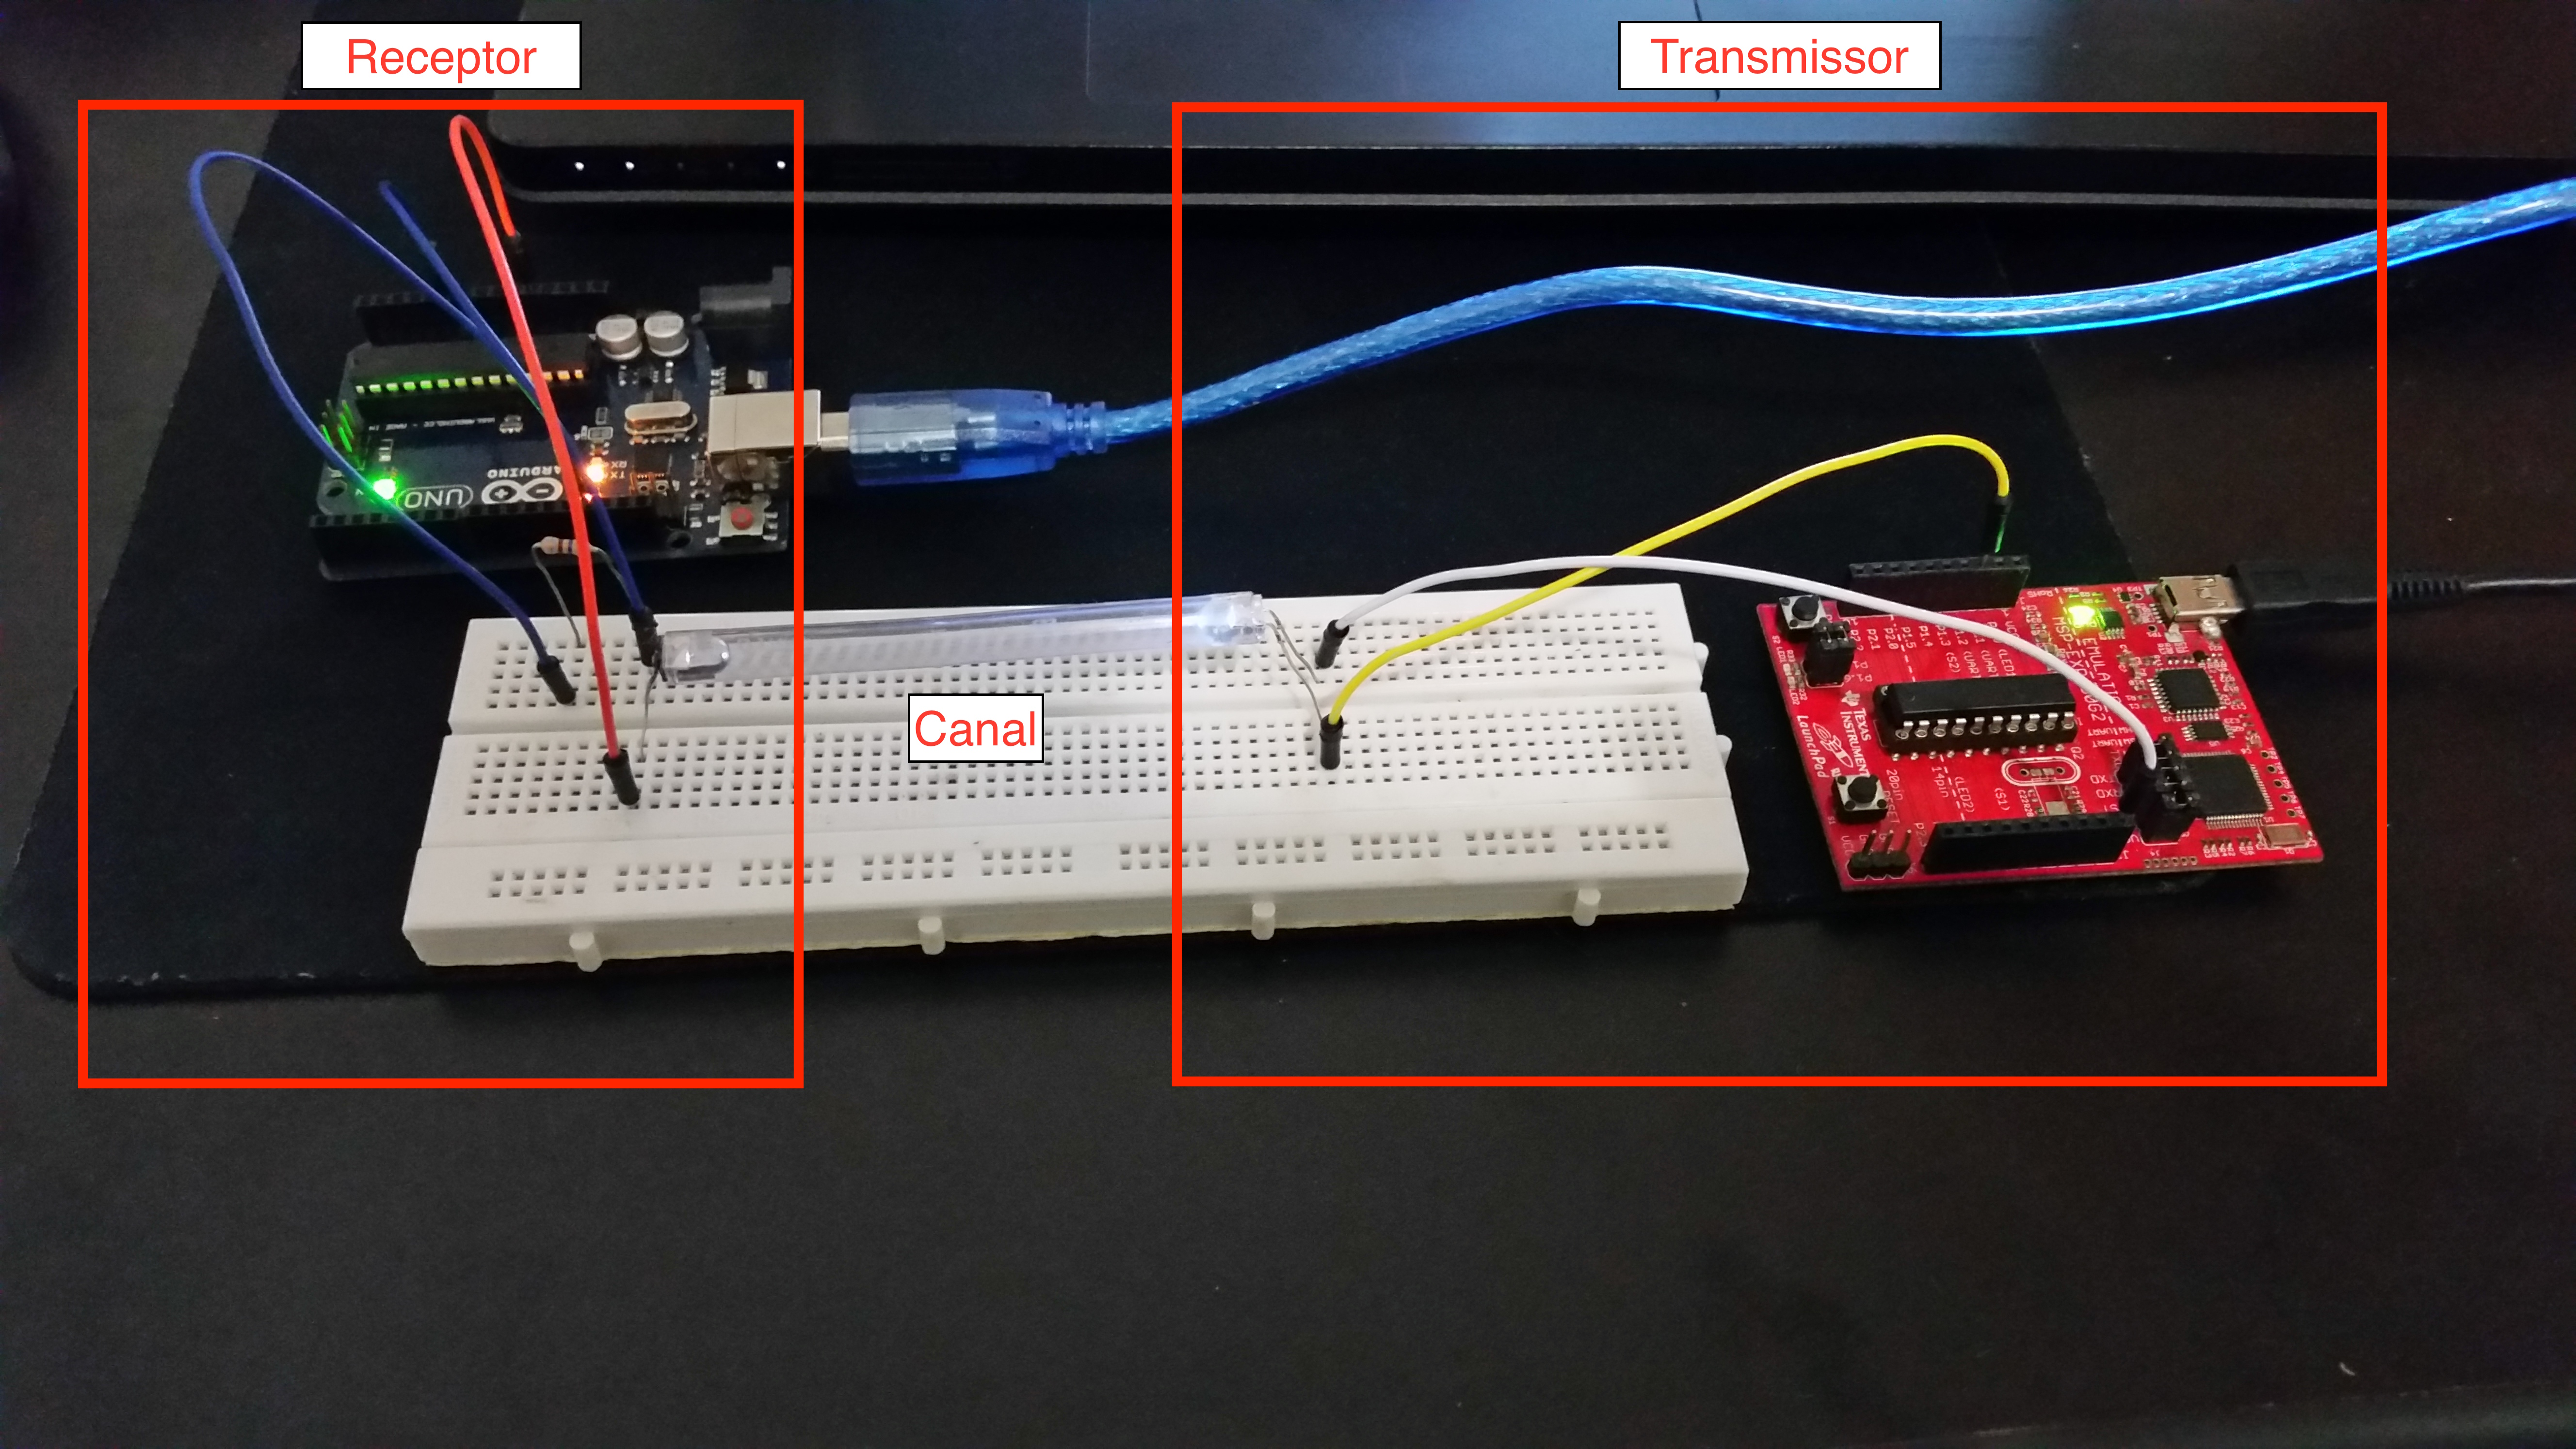
\includegraphics[width = 12cm]{figuras/hardware.jpg}
	\caption{Montagem do \textit{hardware} proposto, receptor a esquerda e transmissor a direita.}
	\label{Fig: Montagem Hardware}
\end{figure}

\subsection{Transmissor}

O sistema de transmissão foi testado a priori visualmente, reduzindo a frequência de envio e comparando com a mensagem. Com a certeza de que a mensagem transmitida está correta, a taxa de transmissão foi expandida para ser testada juntamente ao receptor.

O resistor conectado em série com o diodo LED, foi dimensionado para que o mesmo emita alto brilho sem que o dispositivo queime com o excesso de corrente. Testes mais profundos foram realizados em conjunto com o receptor de dados.

\subsection{Receptor}

Foram realizados testes do receptor direcionado e alinhado com a fonte de fótons. Este experimento se deu em ambiente fechado e com iluminação ambiente e distancia de 7,5 cm. Para excitar o componente óptico foi utilizada a fonte de luz apresentada na figura[\ref{Fig: Montagem Hardware}].

\begin{equation}
	\label{Eq: Conversão AD}
	\frac{Resolução \: ADC}{Voltagem \: do \: Sistema} = \frac{Leitura \: ADC}{Voltagem \: Medida}
\end{equation}

O controlador em uso no receptor trabalha com tensões de até 5v, e seu converso AD possui 10 bits de resolução, o que significa que podemos dividir a voltagem do sistema em 1024 partes.
As leituras realizadas com o LED transmissor ligado ficaram estáveis na faixa dos 875, o que implica que o controlador lê 4,28 v na entrada analógica equação[\ref{Eq: Conversão AD}].
Já com o LED Tx desligado as leituras ficaram nulas, implicando que a luz ambiente não excita tensão na entrada analógica do sistema.

Podemos tomar duas conclusões deste experimento a primeira é que estabelecemos um nível de \textit{threshold} que define se a leitura é de um bit de nível alto ou de um bit de nível baixo, e a segunda conclusão é que o sensor mostrou eficiência na detecção de sinais altos e baixos, apresentando grande diferença entre eles, o que reduz o risco de troca de bis 1 por bits 0.


\subsection{Alinhamento e Área de cobertura}

O alinhamento do sistema e uma parte crucial na transmissão de dados. Visto que o receptor possui estreito ângulo com boa sensibilidade em torno de $10^{\circ}$. No limite destes $10^{\circ}$ a potência que o receptor recebe representa 50\% do sinal em comparação ao recebido utilizando o alinhamento axial. O fato reflete que um conjunto desalinhado torna impossível que haja comunicação entre os sistemas. Para a solucionar o problema, temos algumas alternativas, como adição de refletores e a aquisição de sensores específicos a comunicação não direcional.

Já a área de cobertura, pode ser expandida significativamente com o uso de LED de alta potência presentes no mercado.
Contudo os benefícios tem um custo, e sua viabilidade deve ser analisada.  

\section{Resultados}

O sistema de comunicação VLC funcionou com sucesso, apresentando taxas de erro baixa para frequências menores que 400 Hz apresentado na figura [\ref{Fig: 100Hz}]. Para frequnências acima de 400 Hz há erros consideráveis como apresentado na figura [\ref{Fig: 400Hz}]. A taxa de erro da transmissão aumenta exponencialmente entre os valores maiores que 300 Hz. Fato que pode ser atribuido a limitações de hardware tanto para excitar o led devidamente quanto para detectar o sinal óptico.

As propostas de implementação de \textit{hardware} futuros visam sanar tais limitações e ainda abrir a possibilidade de ampliar a taxa de envio de dados.

Apesar do sistema proposto ser apenas para prova de conceito, e não a versão final, esta tecnologia mostra muito potencial na área de telecomunicações pelo fato de possuir várias áreas de aplicação, além de um grande salto nas taxas de transmissão.

\begin{figure}
	\centering
		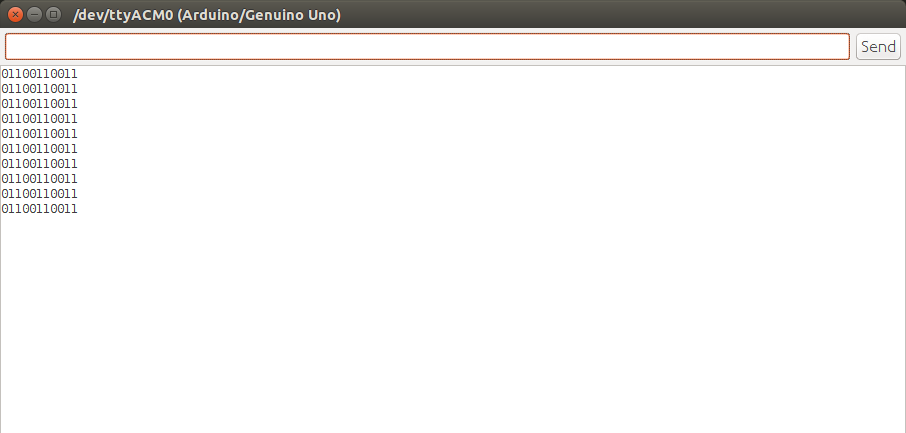
\includegraphics[width = 12cm]{figuras/part4}
	\caption{Detecção dos dados a 100 Hz, sem erros.}
	\label{Fig: 100Hz}
\end{figure}

\begin{figure}
	\centering
		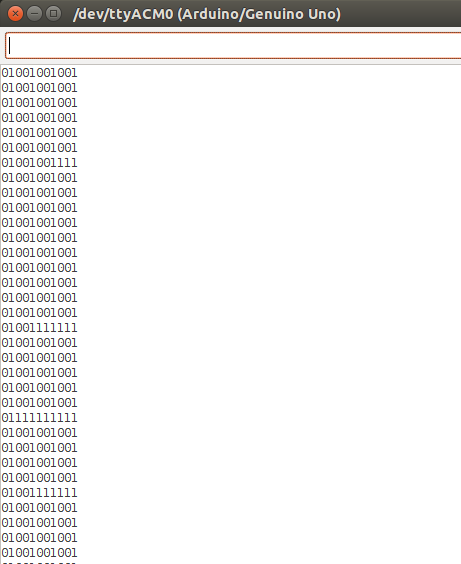
\includegraphics[width = 12cm]{figuras/part5}
	\caption{Dados apresentados na detecção a 400 Hz apresenta erros significativos.}
	\label{Fig: 400Hz}
\end{figure}
